\chapter{Estrutura do Projeto}
\label{sec:estrutura}

  %TODO citation for metaprogramming
  Esse capítulo tem o objetivo de expor o conceito que projetamos para nosso
  sistema. Existe uma certa complexidade em entender como os diversos
  componentes dele se relacionam - principalmente devido ao fato deles usarem
  técnicas como geração de código automatizada e análise reflexiva de código. A
  ideia por trás dessas técnicas também serão explicadas nesse capítulo.
  
  A seção \ref{sec:estrutura:geral} buscará deixar
  claro o contexto em que o projeto funciona e como as responsabilidades da
  solução são distribuídas. As seções \ref{sec:estrutura:opa} e
  \ref{sec:estrutura:opwig} detalham as duas principais partes do projeto, e a
  seção \ref{sec:estrutura:integration}, por fim, explica como tudo isso
  funciona em conjunto para produzir o resultado desejado.

  \section{Visão Geral}
  \label{sec:estrutura:geral}
  
    Um usuário do nosso sistema estará tipicamente desenvolvendo uma aplicação
    em uma linguagem compilada (mais especificamente, \CXX{}) que de alguma
    forma precisa interagir com uma linguagem de \script{}. Essa interação pode
    ser estabelecida diretamente entre elas se a máquina virtual da linguagem de
    \script{} em questão tiver sido programada na linguagem compilada usada,
    pois isso dará acesso:
    
    \begin{itemize}
      \item[(A)]
        À API própria da máquina virtual que permite que ela seja manipulada
        através de sua linguagem nativa.
      \item[(B)]
        Ao protocolo com o qual \script{s} podem pedir à máquina virtual acesso
        a recursos programados na linguagem nativa dela.
    \end{itemize}

    Esses dois elementos estabelecem duas vias de interação entre as linguagens
    envolvidas. Através de (A) a linguagem compilada pode acessar e manipular
    elementos da linguagem de \script{}, enquanto que usando (B) o contrário é
    possível. O propósito do sistema que desenvolvemos é abstrair e automatizar
    o uso dessas duas vias para minimizar o esforço que o usuário necessita para
    desenvolver a interação desejada na sua aplicação.

    \begin{figure}[ht]
      \centering
      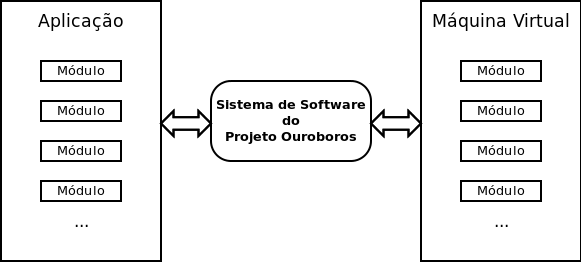
\includegraphics[width=.8\textwidth]{overview-simple.png}
      \caption{Esquematização bem simplificada do sistema.}
      \label{fig:overview-simple}
    \end{figure}

    Vamos dizer que tanto a aplicação quantos os \script{s} estão divididos
    em \textbf{módulos}. Eles serão os objetos das interações tanto do tipo (A)
    quanto do tipo (B), representando o conjunto de elementos provenientes de
    uma ou de outra linguagem que podem ser acessados e manipulados. Por
    exemplo, se a aplicação do usuário for um jogo de ação no qual o jogador
    enfrenta inimigos virtuais, ele poderia usar \script{s} para implementar a
    inteligência artifical desse inimigos, para que fosse fácil ajustá-las sem
    ter que re-compilar o jogo. Desse modo, cada um desses \script{s} seria um
    módulo que a aplicação precisaria carregar e usar durante sua execução.
    Eles, por sua vez, precisariam interagir com módulos da aplicação para que
    as inteligências artificiais conseguissem manipular seus personagens dentro
    do mundo virtual do jogo.

    Dessa forma, uma primeira ilustração bem simplificada da estrutura geral do
    nosso sistema é a representada na Figura \ref{fig:overview-simple}.

  \section{Biblioteca de abstração de APIs de linguagens de \emph{script}.}
  \label{sec:estrutura:opa}
  TODO
  
  \section{Gerador de \emph{wrappers} e interfaces.}
  \label{sec:estrutura:opwig}
  TODO
  
  \section{Integrando e entregando tudo para o usuário.}
  \label{sec:estrutura:integration}
  TODO
